% \usepackage{tabularray}
\begin{table}[H]
\centering
\begin{tblr}{
  row{odd} = {c},
  row{2} = {c},
  cell{1}{1} = {c=2}{},
  cell{4}{2} = {c},
  hlines,
  vlines,
}
Leyenda           &                                                     \\
p                 & Nivel de satisfacción                               \\
g                 & Nivel de importancia de los criterios de evaluación \\
Puntaje del 1 a 4 & 1 la puntuación más baja y 4 la más alta (ideal)    
\end{tblr}
\end{table}

\begin{table}[H]
\centering
 \caption{Evaluación de criterios ténicos}
 \label{Tab:ev_tecnica}
\begin{tblr}{
  row{1} = {c},
  row{2} = {c},
  row{3} = {c},
  row{4} = {c},
  cell{1}{1} = {c=10}{},
  cell{2}{1} = {r=2}{},
  cell{2}{2} = {r=2}{},
  cell{2}{3} = {c=2}{},
  cell{2}{5} = {c=2}{},
  cell{2}{7} = {c=2}{},
  cell{2}{9} = {c=2}{},
  cell{5}{2} = {c},
  cell{5}{3} = {c},
  cell{5}{4} = {c},
  cell{5}{5} = {c},
  cell{5}{6} = {c},
  cell{5}{7} = {c},
  cell{5}{8} = {c},
  cell{5}{9} = {c},
  cell{5}{10} = {c},
  cell{6}{2} = {c},
  cell{6}{3} = {c},
  cell{6}{4} = {c},
  cell{6}{5} = {c},
  cell{6}{6} = {c},
  cell{6}{7} = {c},
  cell{6}{8} = {c},
  cell{6}{9} = {c},
  cell{6}{10} = {c},
  cell{7}{2} = {c},
  cell{7}{3} = {c},
  cell{7}{4} = {c},
  cell{7}{5} = {c},
  cell{7}{6} = {c},
  cell{7}{7} = {c},
  cell{7}{8} = {c},
  cell{7}{9} = {c},
  cell{7}{10} = {c},
  cell{8}{2} = {c},
  cell{8}{3} = {c},
  cell{8}{4} = {c},
  cell{8}{5} = {c},
  cell{8}{6} = {c},
  cell{8}{7} = {c},
  cell{8}{8} = {c},
  cell{8}{9} = {c},
  cell{8}{10} = {c},
  cell{9}{2} = {c},
  cell{9}{3} = {c},
  cell{9}{4} = {c},
  cell{9}{5} = {c},
  cell{9}{6} = {c},
  cell{9}{7} = {c},
  cell{9}{8} = {c},
  cell{9}{9} = {c},
  cell{9}{10} = {c},
  cell{10}{2} = {c},
  cell{10}{3} = {c},
  cell{10}{4} = {c},
  cell{10}{5} = {c},
  cell{10}{6} = {c},
  cell{10}{7} = {c},
  cell{10}{8} = {c},
  cell{10}{9} = {c},
  cell{10}{10} = {c},
  cell{11}{2} = {c=2,r=2}{c},
  cell{11}{4} = {c},
  cell{11}{5} = {r=2}{c},
  cell{11}{6} = {c},
  cell{11}{7} = {r=2}{c},
  cell{11}{8} = {c},
  cell{11}{9} = {r=2}{c},
  cell{11}{10} = {c},
  cell{12}{4} = {c},
  cell{12}{6} = {c},
  cell{12}{8} = {c},
  cell{12}{10} = {c},
  cell{11}{1} = {r},
  cell{12}{1} = {r},
  vlines,
  hline{1-2,4-11,13} = {-}{},
  hline{3} = {3-10}{},
  hline{12} = {1,4,6,8,10}{},
}
Evaluación Técnica           &   &        &      &        &      &        &      &            &    \\
Criterio técnico             & g & Sol. 1 &      & Sol. 2 &      & Sol. 3 &      & Sol. Ideal &    \\
                             &   & p      & gp   & p      & gp   & p      & gp   & p          & gp \\
Conexiones entre componentes & 4 & 3      & 12   & 2      & 8    & 3      & 12   & 4          & 16 \\
Adaptabilidad                & 4 & 2      & 8   & 2      & 8   & 3      & 12   & 4          & 16 \\
Automatización               & 3 & 2      & 6    & 2      & 6    & 3      & 9    & 4          & 12 \\
Seguridad                    & 4 & 4      & 16   & 4      & 16   & 4      & 16   & 4          & 16 \\
Facilidad de uso             & 3 & 3      & 9    & 2      & 6    & 3      & 9    & 4          & 12 \\
Facil ensamble               & 2 & 2      & 4    & 3      & 6    & 3      & 6    & 4          & 8  \\
Consumo de energía           & 3 & 3      & 9    & 3      & 9   & 4      & 12   & 4          & 12 \\
Sumatoria                    &   &        & 64   &        & 59   &        & 76   &            & 92 \\
Xi                           &   &        & 0,69 &        & 0,64 &        & 0,83 &            & 1  
\end{tblr}
\end{table}

\begin{table}[H]
\centering
\caption{Evaluación de criterios económicos}
\label{Tab:ev_economica}
\begin{tblr}{
 row{1} = {c},
 row{2} = {c},
 row{3} = {c},
 cell{1}{1} = {c=10}{},
 cell{2}{1} = {r=2}{},
 cell{2}{2} = {r=2}{},
 cell{2}{3} = {c=2}{},
 cell{2}{5} = {c=2}{},
 cell{2}{7} = {c=2}{},
 cell{2}{9} = {c=2}{},
 cell{4}{2} = {c},
 cell{4}{3} = {c},
 cell{4}{4} = {c},
 cell{4}{5} = {c},
 cell{4}{6} = {c},
 cell{4}{7} = {c},
 cell{4}{8} = {c},
 cell{4}{9} = {c},
 cell{4}{10} = {c},
 cell{5}{2} = {c},
 cell{5}{3} = {c},
 cell{5}{4} = {c},
 cell{5}{5} = {c},
 cell{5}{6} = {c},
 cell{5}{7} = {c},
 cell{5}{8} = {c},
 cell{5}{9} = {c},
 cell{5}{10} = {c},
 cell{6}{2} = {c},
 cell{6}{3} = {c},
 cell{6}{4} = {c},
 cell{6}{5} = {c},
 cell{6}{6} = {c},
 cell{6}{7} = {c},
 cell{6}{8} = {c},
 cell{6}{9} = {c},
 cell{6}{10} = {c},
 cell{7}{2} = {c},
 cell{7}{3} = {c},
 cell{7}{4} = {c},
 cell{7}{5} = {c},
 cell{7}{6} = {c},
 cell{7}{7} = {c},
 cell{7}{8} = {c},
 cell{7}{9} = {c},
 cell{7}{10} = {c},
 cell{8}{2} = {c},
 cell{8}{3} = {c},
 cell{8}{4} = {c},
 cell{8}{5} = {c},
 cell{8}{6} = {c},
 cell{8}{7} = {c},
 cell{8}{8} = {c},
 cell{8}{9} = {c},
 cell{8}{10} = {c},
 cell{9}{1} = {r},
 cell{9}{2} = {c=2,r=2}{c},
 cell{9}{4} = {c},
 cell{9}{5} = {r=2}{c},
 cell{9}{6} = {c},
 cell{9}{7} = {r=2}{c},
 cell{9}{8} = {c},
 cell{9}{9} = {r=2}{c},
 cell{9}{10} = {c},
 cell{10}{1} = {r},
 cell{10}{4} = {c},
 cell{10}{6} = {c},
 cell{10}{8} = {c},
 cell{10}{10} = {c},
 vlines,
 hline{1-2,4-9,11} = {-}{},
 hline{3} = {3-10}{},
 hline{10} = {1,4,6,8,10}{},
}
Evaluación Económica                 &   &        &      &        &      &        &      &           &    \\
Criterio económico                 & g & Sol. 1 &      & Sol. 2 &      & Sol. 3 &      & Sol Ideal &    \\
                                  &   & p      & gp   & p      & gp   & p      & gp   & p         & gp \\
Cantidad de componentes            & 4 & 4      & 16   & 2      & 8    & 3      & 12   & 4         & 16 \\
Costo de componentes electrónicos  & 4 & 3      & 12   & 2      & 8    & 3      & 12   & 4         & 16 \\
Costo de materiales mecánicos      & 3 & 2      & 6    & 4      & 12   & 3      & 9    & 4         & 12 \\
Costo de desarrollo de la interfaz & 4 & 2      & 8    & 2      & 8    & 3      & 12   & 4         & 16 \\
Energía (costo)                    & 2 & 3      & 6    & 2      & 4    & 3      & 6    & 4         & 8  \\
Sumatoria                          &   &        & 46   &        & 37   &        & 51   &           & 68 \\
Xi                                 &   &        & 0,71 &        & 0,59 &        & 0,75 &           & 1  
\end{tblr}
\end{table}

A partir de las tablas, se elaboró un gráfico comparativo para determinar el concepto de solución óptimo, el cual se presenta a continuación en la Figura \ref{fig:eva_t_e_f}
\begin{figure}[H]
   \centering
   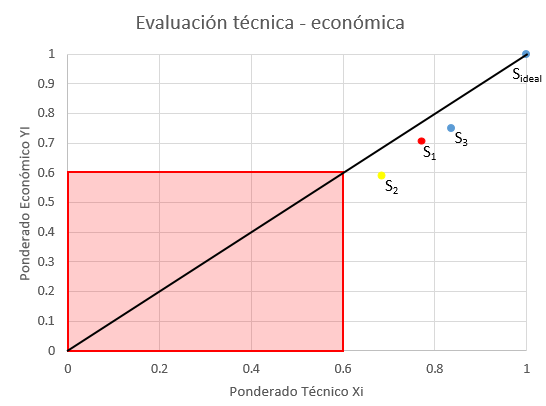
\includegraphics[width=0.8\textwidth]{CHPTRS/CH03_DICON/Fig/EvaluacionT-E.png}
   \caption{Análisis técnico-económico de los conceptos de solución}
   \label{fig:eva_t_e_f}
   \end{figure}


\textbf{Criterios Técnicos:}
\begin{enumerate}
    \item \textbf{Conexión entre componentes}: Se asignó un peso
    de 4 a este criterio, ya que es necesario  que todas las combinaciones de componentes puedan integrarse directamente, sin depender de medios adicionales no especificados para su funcionamiento. En este caso, el principal inconveniente lo presenta la solución 2, ya que está limitada al uso de internet para manejar el \ac{HW}. Además, requiere un microcontrolador con capacidad de conexión a internet, lo que podría incrementar los costos o, en su defecto, demandar componentes adicionales para posibilitar la comunicación con la interfaz.
    
    \item \textbf{Adaptabilidad:}  Se estableció un peso de 4 debido a que una de las principales funcionalidades buscadas en el diseño del estimador es su adaptabilidad a motores en el rango de 12V. Dentro de este rango se encuentran diversos tipos de motores, los cuales no comparten una geometría estándar. Se optará por no utilizar un mecanismo de sujeción automatizada, el ajuste será solucionado utilizando elementos de sujeción como \textit{brackets} a la medida de los motores que cuenten con agujeros de sujeción. Por lo tanto se le designará cómo mayor puntaje a la alternativa 3, y las otras dos soluciones obtendrán  un puntaje de 2 debido a que el motor puede dañarse debido al sobreajuste o si hay algún desperfecto en su mecanismo de control.
    
    \item \textbf{Automatización:}  La automatización en esta solución no será total, se busca que el sistema sea semiautomatizado, priorizando que el único proceso completamente automatizado sea la extracción y el cálculo de parámetros. Por ello, se asignará un peso de 3 a este apartado.
    La solución más difícil de automatizar será aquella que utiliza ajuste por servomotores y correas, debido a que implica la fijación de varios componentes al chasis. Además, el tamaño potencialmente considerable de estos componentes podría extender el área utilizada por el \ac{HW}, lo que podría resultar en el incumplimiento de los requerimientos definidos.
    
    \item \textbf{Seguridad:} El peso elegido de este criterio es 4 debido a la importancia que supone la seguridad del usuario que manipule la máquina. En este caso las 3 soluciones cumplen con esto último por lo que se les asignará un puntaje adecuado a cada una. 
    
    \item \textbf{Facilidad de uso:} Este criterio evalúa qué tan amigable es la máquina para el usuario. Aunque gran parte de esta experiencia depende del diseño de la interfaz, también es importante considerar la forma de fijación del motor. Entre las tres propuestas, la que utiliza servomotores podría presentar cierta complejidad, ya que requiere la sincronización precisa de ambos servos. Esto podría generar inconvenientes técnicos que, eventualmente, demandarían mantenimiento adicional. La del ajuste por apriete tiene el inconveniente de que si algo llegase a fallar se puede dañar al motor. Por último la tercera alternativa es la más segura pero no automatizada.
    
    \item \textbf{Fácil ensamble:} Cuenta con un peso de 2, debido a los materiales con los que se diseñará el chasis que contendrá los componentes. La solución que utiliza chapas metálicas, será la más complicada de ensamblar debido a los detalles que se debe de hacer, de igual forma que el MDF, se necesite comprar componentes adicionales que ayuden a su fijación. 
    
    \item \textbf{Consumo de Energía:} Este criterio evalúa las soluciones considerando elementos que consumen potencia durante periodos prolongados, como los ventiladores, los cuales recibirán un menor puntaje. También se tomarán en cuenta las formas de alimentación del sistema, si se diseñará o se usará una fuente para la conversión de tensión. Sin embargo, dado que estos cambios son manejables, si se diseña correctamente, las variaciones en las puntuaciones no serán significativas.

    
\end{enumerate}

\textbf{Criterios económicos:}
\begin{enumerate}
    \item \textbf{Cantidad de componentes:} Se refiere a la cantidad de componentes que tendrá la máquina a diseñar, se espera que la cantidad de estos no sea elevado debido a que esto incrementaría el presupuesto invertido para la implementación. Se le asignó un peso de 4 debido a la importancia que conlleva esto. También porque si bien se mencionan los componentes, también se debe considerar los procesos de fabricación por los que pasarán estos materiales para obtener una pieza, por ejemplo el chasis o la estructura que contendrá al motor.

    \item \textbf{Costo de componentes electrónicos:} Los componentes electrónicos más costosos son los de regulación de energía, sensores y actuadores (excluyendo el controlador). Entre controladores, las \ac{SBC}s son más caras que los microcontroladores por su mayor capacidad de procesamiento y memoria, ideales para tareas con procesamiento de datos considerable. En regulación, una fuente lineal es significativamente más costosa y menos eficiente que una \textit{switching} por el uso de transformadores (mayor tamaño, peso y costos), por lo que se descarta. En sensores, los ópticos son los más económicos por su diseño sencillo y el uso de \textit{LEDs} infrarrojos y fotodetectores; en cambio, los \textit{encoders} magnéticos, aunque más precisos y resistentes, son más costosos por la complejidad de sus materiales y fabricación.

    
    \item \textbf{Costo de materiales mecánicos:} El análisis se centra principalmente en los materiales que se utilizarán para el chasis y las partes que soportarán los componentes, evaluando tanto el costo de los materiales como el trabajo necesario para la fabricación de estos. El material más económico sería el utilizado en piezas diseñadas con impresión 3D, como el PLA o el ABS, los cuales se comercializan a precios accesibles en función del peso requerido. El principal factor que podría incrementar el costo es el proceso de impresión (ver Anexo \ref{an:Anexo_H}). Por otro lado, el uso de chapa metálica ofrece la ventaja de garantizar que el chasis soportará todas las cargas generadas durante el funcionamiento del motor. Sin embargo, su costo suele ser elevado, especialmente al considerar el trabajo adicional necesario para moldear la chapa según la geometría deseada. Este proceso puede requerir maquinaria especializada, como dobladoras o taladros de banco, lo que aumenta los costos de fabricación. Finalmente, el MDF aparece como una opción que puede ser cortada fácilmente a medida y su precio no es excesivo. No obstante, este material es menos resistente y propenso a fracturarse cuando se somete a fuerzas considerables. Por todo lo expuesto se designa los puntajes en 3 para las soluciones de impresión 3D y chapa metálica, mientras que al que utiliza MDF se le reducirá un punto por temas de estabilidad y resistencia a la carga del motor una vez es energizado.
    
    \item \textbf{Costo de desarrollo de la interfaz:} Se refiere al costo estimado del desarrollo \ac{SW} del sistema. Cuenta con un peso de 4, debido al impacto que se deberá considerar al momento de elegir el entorno de desarrollo de la interfaz solicitada. A la solución 1 se le asignará la menor nota, debido a que utiliza en su totalidad MATLAB para el desarrollo de la solución. En el Anexo \ref{an:Anexo_D}, se muestran los precios de la licencia del programa MATLAB. Por otro lado, la solución 2 también se le restará un punto por ello, ya que utiliza la conexión con un \textit{script} de MATLAB que tendrá el código del estimador de parámetros. La mayor nota, será para la solución 3 al utilizar \ac{SW} que no requiere de un costo adicional para su implementación. Sin embargo, requerirá de un mayor mantenimiento y saberes técnicos si se va a utilizar enteramente entornos de desarrollo gratuitos
    
    \item \textbf{Energía (costo)} : Se refiere al costo que significará usar la máquina que diseñemos. Cuenta con un peso de 2, debido a que los componentes a usar no serán energizados con gran potencia. El consumo de energía de las soluciones planteadas no debería significar un gasto significativo. Los componentes que más energía consumirán son la PC o Laptop que se encargue de la estimación y al momento de energizar al motor para la toma de datos. Además, la tarifa energética para Lima, Perú al momento de escribir el presente trabajo de investigación varía entre S/ 0.50 - S/ 0.70 por el kWh dependiendo del consumo mensual \autocite{Enel_energía}. Como se mencionó en la sección \ref{sec:.lista de req}, la máquina operara un corto tiempo, menor a 2 horas, por lo tanto a todas las soluciones se les designará un puntaje de 3.

\end{enumerate}